\subsection{Driven Simple Harmonic Oscillator with Damping}
The following ODE for a Driven Simple Harmonic Oscillator with Damping represents the dynamic equation governing the motion of a mass subjected to both a restoring force and an external driving force while dissipating energy due to damping.

\subsubsection{Definition}
Let us define a Simple Harmonic Oscillator (SHO) of mass \(m\) and is attached to a spring with spring constant \(k\).
The SHO is subject to a damping force with damping coefficient \(\gamma\) and an additional driving force \(f(t)\).

\vspace{5mm}

Define \(\omega_0 = \sqrt{\frac{k}{m}}\) as the natural frequency of the SHO and the damping force as \(F_d = -2 m \gamma v\), where \(v\) is the velocity of the SHO.

\noindent
Using Newton's Second Law,
\begin{align}
    \Sigma F = ma &= -m \omega_0^2 x - 2 m \gamma v + f(t) \\
    m \frac{d^2 x}{dt^2} &= -m \omega_0^2 x - 2 m \gamma \frac{dx}{dt} + f(t)
\end{align}

\noindent
Dividing by \(m\) and rearranging terms, we get the following differential equation for a driven SHO with damping \citep{Libretexts_2021a}:

\begin{equation} \label{eq:driven_sho_equation}
    \frac{d^2 x}{dt^2} + 2 \gamma \frac{dx}{dt} + \omega_0^2 x(t) = \frac{f(t)}{m}
\end{equation}

\subsubsection{Application of the Fourier Transform}
\noindent
Let us take the Fourier Transform of \cref{eq:driven_sho_equation} with respect to \(t\). Thus, let \(X(\omega)\) and \(F(\omega)\) be the respective Fourier Transforms of \(x(t)\) and \(f(t)\) with respect to \(t\).

\begin{equation}
    \mathcal{F}_t \left\{ \frac{d^2 x}{dt^2} + 2 \gamma \frac{dx}{dt} + \omega_0^2 x(t) \right\} = \mathcal{F}_t \left\{ \frac{f(t)}{m} \right\}
\end{equation}

\noindent
Using \cref{fourier_linearity},
\begin{equation} 
    \mathcal{F}_t \left\{ \frac{d^2 x}{dt^2} \right\} + \mathcal{F}_t \left\{ 2 \gamma \frac{dx}{dt} \right\} + \mathcal{F}_t \left\{ \omega_0^2 x(t) \right\} = \mathcal{F}_t \left\{ \frac{f(t)}{m} \right\}
\end{equation}

\noindent
Using \cref{fourier_scaling},
\begin{equation} 
    \mathcal{F}_t \left\{ \frac{d^2 x}{dt^2} \right\} + 2 \gamma \mathcal{F}_t \left\{ \frac{dx}{dt} \right\} + \omega_0^2 \mathcal{F}_t \left\{ x(t) \right\} = \frac{\mathcal{F}_t \left\{ f(t) \right\}}{m} 
\end{equation}

\noindent
Using \cref{fourier_derivative},
\begin{align}
    \mathcal{F}_t \left\{ \frac{dx}{dt} \right\} &= i \omega \mathcal{F}_t \left\{ x(t) \right\} \\
    &= i \omega X(\omega) + C_1 \\
    \mathcal{F}_t \left\{ \frac{d^2 x}{d t^2} \right\} & = i \omega \mathcal{F}_t \left\{ \frac{dx}{dt} \right\} \\
    & = -\omega^2 X(\omega) + i \omega C_1 + C_2
\end{align}

\noindent
Therefore,
\begin{align}
    -\omega^2 X(\omega) + i \omega C_1 + C_2 + 2 \gamma i \omega X(\omega) + 2 \gamma C_1 + \omega_0^2 X(\omega) = \frac{F(\omega)}{m} \\
    X(\omega) \left( \omega_0^2 - \omega^2 + 2 \gamma i \omega \right) = \frac{F(\omega) - m C_1 \left( i \omega + 2 \gamma \right) - m C_2}{m}
\end{align}

\noindent
Thus,
\begin{equation} \label{eq:driven_sho_fourier}
    X(\omega) = \frac{F(\omega) - m C_1 \left( i \omega + 2 \gamma \right) - m C_2}{m \left( \omega_0^2 - \omega^2 + 2 \gamma i \omega \right)}
\end{equation}

By applying the Fourier Transform to the driven SHO equation, we have reduced the problem from solving a second order ODE (\cref{eq:driven_sho_equation}) to solving a simple algebraic equation (\cref{eq:driven_sho_fourier}). This is a significant reduction in complexity.

Once we have solved for \(X(\omega)\), we can take the inverse Fourier Transform of \cref{eq:driven_sho_fourier} to obtain \(x(t)\) \citep{Libretexts_2021a}.

\begin{align} \label{eq:driven_sho_inverse_fourier}
    x(t) &= \frac{1}{2 \pi} \int_{-\infty}^{\infty} X(\omega) e^{i \omega t} d\omega \\
    &= \frac{1}{2 \pi} \int_{-\infty}^{\infty} \frac{F(\omega) - m C_1 \left( i \omega + 2 \gamma \right) - m C_2}{m \left( \omega_0^2 - \omega^2 + 2 \gamma i \omega \right)} d\omega
\end{align}

\subsubsection{Initial and Boundary Conditions}
\noindent
To constrain the solution of our ODE, we must provide initial and boundary conditions for the ODE. First, we will set the position of the SHO initially at 0.5 units above the equilibrium point. The following condition represents this:
\begin{align}
    x(0)=0.5 \label{eq:driven_sho_equation_initial_condition}
\end{align}

\noindent
For sake of example, a non-periodic driving force as defined below will be utilized:
\begin{align}
    f(t) = e^{-\frac{t}{500}}
\end{align}

\noindent
Let us also apply a boundary condition to allow the SHO to start at rest.
\begin{align}
    x'(0) = 0
\end{align}

\subsubsection{Numerical Solution to Driven SHO}
\cref{eq:driven_sho_inverse_fourier} can be easily solved numerically using the Fast Fourier Transform (FFT) and the Inverse Fast Fourier Transform (IFFT) algorithms. The FFT and IFFT algorithms are optimized algorithms for computing the Discrete Fourier Transform (DFT) and the Inverse Discrete Fourier Transform (IDFT) of a sequence. The Python code can be found in \cref{code:driven_sho}.

\begin{figure}[H]
    \centering
    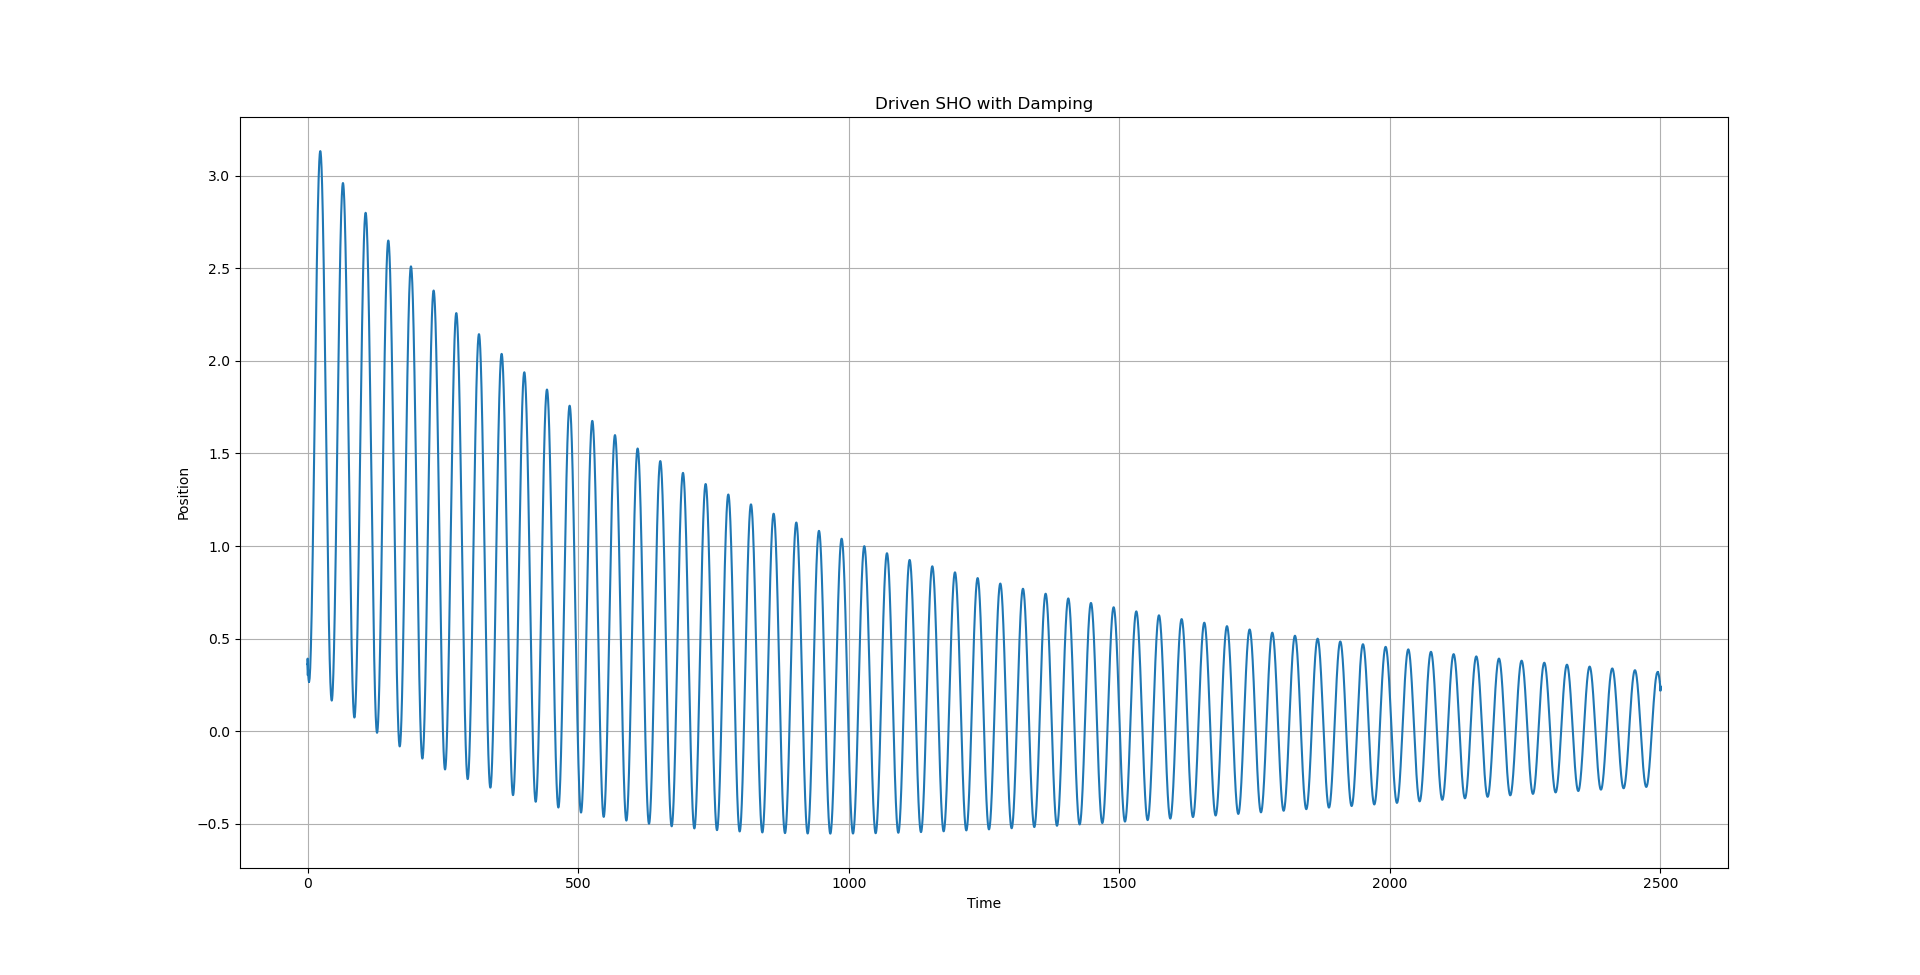
\includegraphics[width=100mm,height=\textheight,keepaspectratio]{images/driven_sho_equation_numerical.png}
    \caption{Defining \cref{eq:driven_sho_equation_initial_condition} as the initial condition, above is the solution to the driven SHO equation with damping using the FFT and IFFT algorithms in Python.}
    \label{fig:driven_sho_equation_numerical}
\end{figure}